\documentclass[12pt]{article}
\usepackage{libertine}
\usepackage[a4paper, left = 2.5cm,right = 2.5cm,top = 2.5cm,bottom = 3cm]{geometry}
\usepackage[english,russian]{babel}
\usepackage{amsmath}
\usepackage{amssymb}
\usepackage{amsfonts}
\usepackage[final]{graphicx}
\usepackage[linktocpage=true, colorlinks=true, linkcolor = blue, citecolor = red]{hyperref}
\usepackage{cmap}
\usepackage{xfrac}
\usepackage[titletoc]{appendix}
\usepackage{pgfplots}
\newcommand{\eprint}{}

\linespread{1.2}

\newcommand{\bq}{\begin{equation}}
\newcommand{\eq}{\end{equation}}

\usepackage{tikz}
%%%%%%%%

\title{Explisit isometric embeddings of collapsing black hole}
\author{A.D. Kapustin, S.A. Paston \\ Saint-Petersburg state university, Saint-Petersburg, Russia}
\date{}
\begin{document}

\maketitle
\begin{abstract}
В этой работе ищутся явные вложения наименьшей размерности для метрики коллапсирующего сферически симметричного облака пылевидной материи, образующего Шварцшильдовскую черную дыру. В работе рассматриваются два подхода, в одном из которых находится глобальное семимерное вложение с изломом, а в другом локальное семимерное, также содержащее излом. Однако для частного случая во втором подходе удается найти гладкое шестимерное вложение, покрывающее все области многообразия.
\end{abstract}

\clearpage

\section{Введение}
Как известно, любое риманово многообразие размерности $d$ может быть изометрически вложено в плоское объемлющее пространство размерности $N \geqslant \frac{d(d+1)}{2}$ как минимум локально \cite{gane, kart, fridman61}. В таком случае можно описывать многообразие набором функций вложения $y^a(x)$, а метрику считать индуцированной
\bq
	g_{\mu \nu} = \partial_{\mu} y^a \partial_{\nu} y^b \eta_{ab}.
\eq

Такой подход может оказаться наглядным и полезным для изучения структуры многообразия, однако для этого требуется отыскание явного вида функций вложения. Изучение структуры многообразия очень актуально в отношении черных дыр, так как соответствующие им многообразия часто имеют нетривиальную структуру. Кроме того, отыскание явных вложений геометрии черных дыр является важной задачей с точки зрения формулировки гравитации Редже-Тейтельбойма \cite{regge}.

Сложность заключается в том, что для четырехмерного пространства-времени в случае общего положения задача отыскания явного вида функций вложения это система $10$ уравнений в частных производных с $4$ независимыми переменными. Задача облегчается, если у многообразия присутствуют дополнительные симметрии. Если этих симметрий достаточно, то существует конструктивный метод упрощения задачи вплоть до решения системы ОДУ. В частности, таким образом были найдены и проклассифицированы вложения наименьшей размерности для Шварцшильдовских черных дыр \cite{statja27}.  

Физически интересным оказывается случай, в котором глобальная симметрия многообразия оказывается меньшей, чем симметрия Шварцшильдовой черной дыры. Речь идет о коллапсе, при котором облако материи сжимается, образуя черную дыру динамически. В этой задаче происходит образование горизонта, что было бы интересно пронаблюдать на языке вложеной поверхности. Предлагается рассмотреть наиболее простой случай коллапса, в котором считать материю пылевидной, а ее распределение сферически симметричным.
\section{Выбор координат для описания коллапса}
Для описания движения пылевидной материи кажется разумным использовать систему синхронных сопутствующих координат, а, в силу сферической симметрии, в качестве двух пространственных следует выбрать углы $\theta$ и $\varphi$. Оставшиеся координаты обозначим $\tau$ и $\chi$. Метрика решения для произвольного распределения материи задается линейным элементом вида
\bq
\label{metric}
	d s^2 = d \tau^2 - \frac{(r'(\tau, \chi))^2}{1+f(\chi)} d\chi^2 - r^2(\tau, \chi) d \Omega,
\eq
где функция $r(\tau, \chi)$ определяется одним из трех способов
\bq
	r(\tau, \chi) = \left\{
	\begin{matrix}
	\frac{F(\chi)}{2 f(\chi)} H \left( \frac{2(f(\chi))^{\sfrac{3}{2}} }{F(\chi)}(\tau_0(\chi)-\tau)  \right) , \ \ \ \ f(\chi) > 0\\
	\left( \frac{9F(\chi)}{4} \right)^{\sfrac{1}{3}} \left[ \tau_0(\chi)- \tau \right]^{\sfrac{2}{3}}, \ \ \ \ f(\chi) = 0 \\
	- \frac{F(\chi)}{2 f(\chi)} E \left( \frac{2(-f(\chi))^{\sfrac{3}{2}} }{F(\chi)}(\tau_0(\chi)-\tau) \right), \ \ \ \ f(\chi) < 0  
	\end{matrix} \right.
\eq
Функции $E(x)$ и $H(x)$  служат для обращения параметрических зависимостей
\bq
	\begin{array}{c}
	E = 1 - \cos{\eta}, \\
	x = \eta - \sin{\eta},
	\end{array} \ \ \ \ \ \ \ \
	\begin{array}{c}
	H = \ch{\eta}-1, \\
	x = \sh{\eta} - \eta,
	\end{array}
\eq
а функции $F(\chi), f(\chi)$ и $\tau_0(\chi)$ задают распределение плотности материи и начальные скорости \cite{landau}.

Если потребовать однородности распределения материи в начальный момент, то пространство внутри коллапсирующего шара будет описываться геометрией открытой, пространственно-плоской или закрытой модели Фридмана соответственно выбору первого, второго или третьего способа определения $r(\tau, \chi)$. Внешнее к шару пространство, согласно теореме Биркгофа, во всех случаях описывается геометрией Шварцшильда. Метрика будет иметь координатную особенность в виде скачка на границе шара, которую можно устранить переходом к координатам $(\tau, r, \theta, \varphi)$, что будет использовано в одном из подходов. 

\section{Случай с пространственно-плоской моделью Фридмана}

Произведем описанную выше замену координат. Тогда метрика общего вида (\ref{metric}) перейдет в 
\bq
	d s^2 = \left( 1- \frac{\dot{r}^2}{1+f(\chi)}\right) d \tau^2 + 2\frac{\dot{r}}{1+f(\chi)}dr d\tau - \frac{dr^2}{1+f(\chi)} - r^2 d\Omega.
\eq
Если теперь выбрать $f(\chi)=0$, то $r(\tau, \chi)$ выразится через элементарные функции и можно вычислить $\dot{r} = \frac{\partial r(\tau, \chi)}{\partial \tau}$. После всех преобразований метрика примет вид
\bq
\label{metric2}
	d s^2 = \left(1-\frac{4F(\tau, r)}{9 r} \right)d\tau^2 - 2 \frac{3}{2}\sqrt{\frac{F(\tau, r)}{r}}dr d\tau  - dr^2 - r^2 d\Omega.
\eq
Как уже упоминалось, выбор $f(\chi)=0$ соответствует тому, что часть пространства, содержащая материю описывается пространственно-плоской моделью Фридмана.

Чтобы метрика (\ref{metric2}) отвечала однородной плотности материи в шаре, следует выбрать
\bq
	F(\tau, r) = \min{ \left( \frac{r^3}{(1-\tau)^2}, F_0 \right) }.
\eq
Тогда видно, что метрика оказывается непрерывной, однако не всюду дифференцируемой функцией.

\begin{figure}[h!]
	\centering
	\begin{tikzpicture}[scale=0.75]
		\draw[->] (-5, 0) -- (5, 0)node[below]{$u$};
		\draw[->] (0, -5) -- (0, 5)node[left]{$v$};
		%%
		\draw[->] (4.5, 0.5) -- (5.5, 0.5)node[midway,above]{$r \to \infty$};
		%%
		\begin{scope}
		\clip (7.5, 6) -- (5, 6) -- (0.6, 2.8) .. controls (1, 1) and (1, 0) .. (5, -3) -- (5, -6) -- (7.5, -6) -- cycle;
		\draw[thick, dashed] (-5, -5) -- (5, 5)node[above right]{$r = R$};
		\draw[thick, dashed] (-5, 5) -- (5, -5);
		%%
		\draw (5, 4.9) .. controls (0, 0) and (0, -0) .. (5, -4.9);
		\draw (5, 4.7) .. controls (1.5, 1) and (1.5, -1) .. (5, -4.7);
		\draw (5, 4.5)node[below right]{$r=const$} .. controls (3, 1.5) and (3, -1.5) .. (5, -4.5);
		%%
		\draw (-5, 4.9) .. controls (0, 0) and (0, -0) .. (-5, -4.9);
		\draw (-5, 4.7) .. controls (-1.5, 1) and (-1.5, -1) .. (-5, -4.7);
		\draw (-5, 4.5) .. controls (-3, 1.5) and (-3, -1.5) .. (-5, -4.5);
		%%
		\draw (4.9, 5) .. controls (0, 0) and (0, 0) .. (-4.9, 5);
		\draw (4.8, 5) .. controls (1, 1) and (-1, 1) .. (-4.8, 5);
		\draw[ultra thick] (4.7, 5) .. controls (2, 2) and (-2, 2) .. (-4.7, 5);
		%%
		\draw (4.9, -5) .. controls (0, 0) and (0, 0) .. (-4.9, -5);
		\draw (4.8, -5) .. controls (1, -1) and (-1, -1) .. (-4.8, -5);
		\draw[ultra thick] (4.7, -5) .. controls (2, -2) and (-2, -2) .. (-4.7, -5);
		\draw (0, -3)node[below right]{$r = 0$};
		%%
		\end{scope}
		\draw (0, 3)node[above right]{$r = 0$};
		\draw[blue, very thick] (5, -3) .. controls (1, 0) and (1, 1) .. (0.6, 2.8);
	\end{tikzpicture}
	\caption{\label{infkrusk}The Kruskal diagram for matter collapsing from infinity.}
\end{figure} 

Можно представить область пространства, соответствующую константе $F_0$, на диаграмме Крускала \ref{infkrusk}. Она ограничена мировой линией частицы, лежащей на границе сферы. Для этого случая характерно то, что коллапс происходит с бесконечности, в отличие от второго подхода. Оставшаяся часть многообразия описывается метрикой Фридмана и может быть восстановлена с помощью построеного вложения.

\subsection{Построение вложения для полученной метрики}

Если ввести переменные $t = (1-\tau)^{\sfrac{2}{3}}$ и $p = \frac{r^3}{(1-\tau)^{\sfrac{4}{3}}}$, метрика примет вид
\bq
	d s^2 = \left(\alpha t +f(p) \right) dt^2 + h(p) t \ dp dt - \left(dr(t,p)\right)^2 - r^2(t,p) d \Omega,
\eq
где 
\[
\alpha = \frac{9}{4},\ \ \ \  f(p) = 2 F(p)^{\sfrac{1}{2}} p^{\sfrac{1}{6}} - F(p) p^{-\sfrac{1}{3}}, \ \ \ \  h(p) = \frac{2F(p)^{\sfrac{1}{2}}}{3p^{\sfrac{5}{6}}}.
\]

Если в качестве трех функций вложния выбрать блок $(r \cos{\theta},r \sin{\theta}\cos{\varphi},r \sin{\theta}\sin{\varphi})$, то останется вложить метрику
\bq
	d s^2 = \left(\alpha t +f(p) \right) dt^2 + h(p) t \ dp dt.
\eq
Видно, что ее компоненты являются полиномами по переменной $t$. Тогда можно искать решение уравнений вложения также в виде полиномов. Удобнее всего это сделать в светоподобных координатах объемлющего пространства. Решение представимо в виде
\begin{align}
	y^{+} &= t^3 - \frac{\alpha}{4}t^2-\frac{f(p)}{2}t, \\
	y^1 &= \sqrt{\frac{3}{2}}t^2 + \frac{1}{\sqrt{6}}\int h(p)dp - \frac{1}{2\sqrt{6}}f(p), \\
	y^{-} &= t, \\
	y^{3} &= \frac{1}{\sqrt{6}}\int h(p)dp - \frac{1}{2\sqrt{6}}f(p).
\end{align}
Чтобы получить полный набор функций вложения нужно дописать блок
\begin{align}
	y^4 &= p^{\sfrac{1}{3}}t \cos{\theta}, \\
	y^5 &= p^{\sfrac{1}{3}}t \sin{\theta} \cos{\varphi}, \\
	y^6 &= p^{\sfrac{1}{3}}t\sin{\theta} \sin{\varphi}.
\end{align}

Итого, если вернуться к более естественным переменным, получится набор функций вложения
\begin{align}
	y^{+} &= (\tau')^2 - \frac{\alpha}{4}(\tau')^{\sfrac{4}{3}}-\frac{f\left(\frac{r^3}{(\tau')^2}\right)}{2}(\tau')^{\sfrac{2}{3}}, \\
	y^1 &= \sqrt{\frac{3}{2}}(\tau')^{\sfrac{4}{3}} + \frac{1}{\sqrt{6}}\int \limits_C^{\frac{r^3}{(\tau')^2}} h(p)dp - \frac{1}{2\sqrt{6}}f\left( \frac{r^3}{(\tau')^2}\right), \\
	y^{-} &= (\tau')^{\sfrac{2}{3}}, \\
	y^{3} &= \frac{1}{\sqrt{6}}\int \limits_C^{\frac{r^3}{(\tau')^2}} h(p)dp - \frac{1}{2\sqrt{6}}f\left( \frac{r^3}{(\tau')^2}\right),  \\
	y^4 &= r \cos{\theta}, \\
	y^5 &= r \sin{\theta} \cos{\varphi},  \\
	y^6 &= r \sin{\theta} \sin{\varphi},
\end{align}
где $\tau'$ можно воспринимаь как собственное время частиц, оставшееся до падения на сингулярность.

Таким образом, вложение получается семимерным с сигнатурой $(+,+,-,-,-,-,-)$. Оно, однако, содержит излом, так как выражается через функцию $F(p)$, которая является лишь непрерывной. 

\section{Случай закрытой модели Фридмана}

В рамах второго подхода мы будем работать в сопутствующей системе координат, несмотря на наличие координатной особенности метрики, и попробуем совершить сшивку уже известных вложений для метрики Фридмана и Шварцшильда. 

В сопутствующих координатах уравнение движения метерии имеет вид $\chi = const$, поэтому можно сказать, что область $0 \leqslant \chi < \chi_0$ содержит материю, область $\chi > \chi_0$ соответствует пустому пространству, а $\chi = \chi_0$ --- граница пылевидного шара.

Выберем $r(\tau, \chi)$ согласно третьему способу. Тогда при выборе функций $F, f, \tau_0$, отвечающему постоянной плотности, получится функция
\bq
	r(\tau, \chi) = \frac{R \sin{\chi}}{2 \sin^3{\chi_0}} \cdot E \left( \pi - \frac{2 \sin^3{\chi_0}}{R} \tau \right), \ \ \ \ \text{при } 0 \leqslant \chi < \chi_0, 
\eq
дающая метрику Фридмана
\bq
	ds^2 = d\tau^2 - a^2(\tau) \left(d\chi^2 + \sin^2{\chi}d\Omega \right)
\eq
с $a(\tau) = \frac{R}{2 \sin^3{\chi_0}} E \left( \pi - \frac{2 \sin^3{\chi_0}}{R} \tau \right)$, и
\bq
	r(\tau, \chi) = \frac{r_m(\chi)}{2}\cdot E \left( \pi - \frac{2R^{\sfrac{1}{2}}}{r^{\sfrac{3}{2}}_m(\chi)} \tau \right), \ \ \ \ \text{при } \chi > \chi_0,  
\eq
дающая метрику Шварцшильда. Параметр $\chi_0$ определяет максимальный размер шара. Функция $r_m(\chi)$ содержит произвол, ограничивающийся лишь требованием непрерывности $r(\tau, \chi)$ и стремлением $r_m \to \infty$ при $\chi \to \infty$.

Область $\chi > \chi_0$ может также быть представлена на диаграмме Крускала \ref{closedkrusk}. По ней видно, что в этом случае крайняя и все внутренние частицы материи вылетают из белой сингулярности, достигают максимального удаления и коллапсируют в черную сингулярность. Остальная часть многообразия описывается геометрией Фридмана, как и в предыдущем случае.
\begin{figure}[h!]
	\centering
		\begin{tikzpicture}[scale=0.75]
			\draw[->] (-5, 0) -- (5, 0)node[below]{$u$};
			\draw[->] (0, -5) -- (0, 5)node[left]{$v$};
			%%
			\draw[->] (4.5, 0.5) -- (5.5, 0.5)node[midway,above]{$r \to \infty$};
			%%
			\begin{scope}
			\clip (7.5, 6) -- (5, 6) -- (0, 3.5) .. controls (0, 1) and (1, 0.5) .. (1, 0) -- (1, 0) .. controls (1, -0.5) and (0, -1) .. (0, -3.5) -- (5, -6) -- (7.5, -6) -- cycle;
			\draw[thick, dashed] (-5, -5) -- (5, 5)node[above right]{$r = R$};
			\draw[thick, dashed] (-5, 5) -- (5, -5);
			%%
			\draw (5, 4.9) .. controls (0, 0) and (0, -0) .. (5, -4.9);
			\draw (5, 4.7) .. controls (1.5, 1) and (1.5, -1) .. (5, -4.7);
			\draw (5, 4.5) .. controls (3, 1.5) and (3, -1.5) .. (5, -4.5)node[above right]{$r=const$};
			%%
			\draw (-5, 4.9) .. controls (0, 0) and (0, -0) .. (-5, -4.9);
			\draw (-5, 4.7) .. controls (-1.5, 1) and (-1.5, -1) .. (-5, -4.7);
			\draw (-5, 4.5) .. controls (-3, 1.5) and (-3, -1.5) .. (-5, -4.5);
			%%
			\draw (4.9, 5) .. controls (0, 0) and (0, 0) .. (-4.9, 5);
			\draw (4.8, 5) .. controls (1, 1) and (-1, 1) .. (-4.8, 5);
			\draw[ultra thick] (4.7, 5) .. controls (2, 2) and (-2, 2) .. (-4.7, 5);
			\draw (0, 3)node[above right]{$r = 0$};
			%%
			\draw (4.9, -5) .. controls (0, 0) and (0, 0) .. (-4.9, -5);
			\draw (4.8, -5) .. controls (1, -1) and (-1, -1) .. (-4.8, -5);
			\draw[ultra thick] (4.7, -5) .. controls (2, -2) and (-2, -2) .. (-4.7, -5);
			\draw (0, -3)node[below right]{$r = 0$};
			%%
		%	\draw[blue, thick] (5, -3)node[above right]{$r_m(t)$} .. controls (1, 0) and (1, 1) .. (0.6, 2.8);
			\end{scope}
			\draw[very thick, blue] (0.03, 2.77) .. controls (0.1, 1) and (1, 0.5) .. (1, 0) -- (1, 0) .. controls (1, -0.5) and (0.1, -1) .. (0.03, -2.77);
		\end{tikzpicture}
	\caption{\label{closedkrusk}The Kruskal diagram for the collapse of matter, which flew out of the white singularity.}
\end{figure} 

\subsection{Построение вложения в общем случае}
Согласно \cite{kasner2}, минимальная размерность вложения для метрики Шварцшильда равна~$6$, поэтому известные пятимерные вложения для метрики Фридмана (можно найти в \cite{statja29} или \cite{rosen65, robertson1933}) следует модифицировать добавлением дополнительных функций вложения. Основная идея заключается в том, чтобы <<не трогать>> зависимость функций вложения от координаты $\chi$, а добавить только функции, зависящие от $\tau$.  

Пятимерное вложение метрики Фридмана имеет вид
\begin{align}
	y^0 &= f(\tau), \\
\label{0}	y^1 &= a(\tau) \cos{\chi}, \\
\label{1}	y^2 &= a(\tau) \sin{\chi} \cos{\theta}, \\
\label{2}	y^3 &= a(\tau) \sin{\chi} \sin{\theta} \cos{\varphi}, \\
\label{3}	y^4 &= a(\tau) \sin{\chi} \sin{\theta} \sin{\varphi}.
\end{align}
Функция $y^0$ будет изменена, а оставшийся блок мы договорились оставить без изменений. Тогда при $\chi = \chi_0$ этот блок должен совпадать с какими-нибудь четыремя функциями вложения метрики Шварцшильда. 

Выберем для сшивки какое-либо известное вложение метрики Шварцшильда, содержащее блок
\begin{align}
	&r \cos{\theta}, \\
	&r \sin{\theta} \cos{\varphi}, \\
	&r \sin{\theta} \sin{\varphi}.
\end{align}
Он совпадет на границе с (\ref{1}) --- (\ref{3}), но функция (\ref{0}) в общем случае не совпадет ни с какой из известных функций вложения. Поэтому искуственно добавим еще одну функцию $y^6 = r \ctg{\chi_0}$ к вложению метрики Шварцшильда, расширив его до семимерного. Это было сделано для вложения Фронсдала и обнаружено, что оно перестает покрывать область с большими значениями $r$. При остальных значениях $r$ оно существует и имеет вид
\begin{align}
\label{4}	&y^0 = y^0(t(\tau, \chi), r(\tau, \chi)), \\
\label{5}	&y^1 = y^1(t(\tau, \chi), r(\tau, \chi)), \\
\label{6}	&y^2 = y^2(t(\tau, \chi), r(\tau, \chi)), \\
	&y^3 = r(\tau, \chi) \cos{\theta}, \\
	&y^4 = r(\tau, \chi) \sin{\theta} \cos{\varphi}, \\
	&y^5 = r(\tau, \chi) \sin{\theta} \sin{\varphi}, \\
\label{7}	&y^6 = r(\tau, \chi) \ctg{\chi_0}.
\end{align}

Возвращаясь к вложению метрики Фридмана, следует заменить функцию $f(\tau)$ на блок (\ref{4}) --- (\ref{6}) функций известного вида, взятых при фиксированном значении $\chi = \chi_0$. Всилу того, что оставшийся набор функций вложения совпадает на границе, и компонента $g_{00}$ метрики в обоих областях равна $1$, получившийся набор
\begin{align}
	&y^0 = y^0(t(\tau, \chi_0), r(\tau, \chi_0)), \\
	&y^1 = y^1(t(\tau, \chi_0), r(\tau, \chi_0)), \\
	&y^2 = y^2(t(\tau, \chi_0), r(\tau, \chi_0)), \\
	&y^3 = a(\tau) \sin{\chi} \cos{\theta}, \\
	&y^4 = a(\tau) \sin{\chi} \sin{\theta} \cos{\varphi}, \\
	&y^5 = a(\tau) \sin{\chi} \sin{\theta} \sin{\varphi}, \\
	&y^6 = a(\tau) \cos{\chi}.
\end{align}
является вложением метрики Фридмана в семимерное пространство. 

Сшивка полученного вложения с вложением (\ref{4}) --- (\ref{7}) задает непрерывную поверхность в пространстве с сигнатурой $(+, -, -, -, -, -, -)$, которая имеет излом на границе  $\chi = \chi_0$ и покрывает лишь область конечных $r$. 

\subsection{ Построение вложения в случае $\chi_0 = \frac{\pi}{2}$}

В этом случае максимальный радиус шара $r_{max} = \frac{R}{\sin^2{\chi_0}}$ оказывается равным радиусу шварцшильда $R$. Во время движения материя не выходит из под горизонта, а значит и сшивка будет происходить при значениях $r \leqslant R$.

\begin{figure}[h!]
\centering
\begin{tikzpicture}[scale=0.75]
	\draw[->] (-5, 0) -- (5, 0)node[below]{$u$};
	\draw[->] (0, -5) -- (0, 5)node[left]{$v$};
	%%
	\draw[->] (4.5, 0.5) -- (5.5, 0.5)node[midway,above]{$r \to \infty$};
	%%
	\begin{scope}
	\clip (7.5, 6) -- (5, 6) -- (0, 3.5) .. controls (0, 1) and (0, 0.5) .. (0, 0) -- (0, 0) .. controls (0, -0.5) and (0, -1) .. (0, -3.5) -- (5, -6) -- (7.5, -6) -- cycle;
	\draw[thick, dashed] (-5, -5) -- (5, 5)node[above right]{$r = R$};
	\draw[thick, dashed] (-5, 5) -- (5, -5);
	%%
	\draw (5, 4.9) .. controls (0, 0) and (0, -0) .. (5, -4.9);
	\draw (5, 4.7) .. controls (1.5, 1) and (1.5, -1) .. (5, -4.7);
	\draw (5, 4.5) .. controls (3, 1.5) and (3, -1.5) .. (5, -4.5)node[above right]{$r=const$};
	%%
	\draw (-5, 4.9) .. controls (0, 0) and (0, -0) .. (-5, -4.9);
	\draw (-5, 4.7) .. controls (-1.5, 1) and (-1.5, -1) .. (-5, -4.7);
	\draw (-5, 4.5) .. controls (-3, 1.5) and (-3, -1.5) .. (-5, -4.5);
	%%
	\draw (4.9, 5) .. controls (0, 0) and (0, 0) .. (-4.9, 5);
	\draw (4.8, 5) .. controls (1, 1) and (-1, 1) .. (-4.8, 5);
	\draw[ultra thick] (4.7, 5) .. controls (2, 2) and (-2, 2) .. (-4.7, 5);
	\draw (0, 3)node[above right]{$r = 0$};
	%%
	\draw (4.9, -5) .. controls (0, 0) and (0, 0) .. (-4.9, -5);
	\draw (4.8, -5) .. controls (1, -1) and (-1, -1) .. (-4.8, -5);
	\draw[ultra thick] (4.7, -5) .. controls (2, -2) and (-2, -2) .. (-4.7, -5);
	\draw (0, -3)node[below right]{$r = 0$};
	%%
%	\draw[blue, thick] (5, -3)node[above right]{$r_m(t)$} .. controls (1, 0) and (1, 1) .. (0.6, 2.8);
	\end{scope}
	\draw[ultra thick, blue] (0, 2.77) .. controls (0, 1) and (0, 0.5) .. (0, 0) -- (0, 0) .. controls (0, -0.5) and (0, -1) .. (0, -2.77);
\end{tikzpicture}
\caption{\label{speckrusk}The Kruskal diagram for the special case in which matter does not leave the limits of the Schwarzschild radius}
\end{figure}

Рассмотрим явный вид вложения Фронсдала (можно найти в \cite{statja27,statja29} или \cite{frons})
\begin{align}
\label{8}	y^0 & = 2 R \sqrt{\frac{R}{r(\tau, \chi)}-1} \cdot \ch{\left( \frac{t(\tau, \chi)}{2 R}\right)},  \\
	y^1 & = 2 R \sqrt{\frac{R}{r(\tau, \chi)}-1} \cdot \sh{\left( \frac{t(\tau, \chi)}{2 R}\right)},  \\
\label{9}	y^2 & = R \cdot q \left( \frac{r(\tau, \chi)}{R} \right), \\
	y^3 &= r(\tau, \chi) \cos{\theta},  \\
	y^4 &= r(\tau, \chi) \sin{\theta} \cos{\varphi},  \\
	y^5 &= r(\tau, \chi) \sin{\theta} \sin{\varphi}. 
\end{align}

Оказывается, что $t(\tau, \frac{\pi}{2}) \equiv 0$, поэтому $y^1$ на границе сшивки обнуляется, как и функция (\ref{0}) во вложении метрики Фридмана. Получается, что в этом случае нет необходимости расширять вложение Фронсдала до семимерного, а во вложении метрики Фридмана достаточно заменить $f(\tau)$ на две функции  (\ref{8}), (\ref{9}), взятые при $\chi = \frac{\pi}{2}$. Интересно, что в этом случае после сшивки вложение получается гладким и покрывает все значения $r>0$. Вложение оказывается шестимерным с сигнатурой $(+, -, -, -, -, -)$.

\begin{figure}[h!]
	\centering
	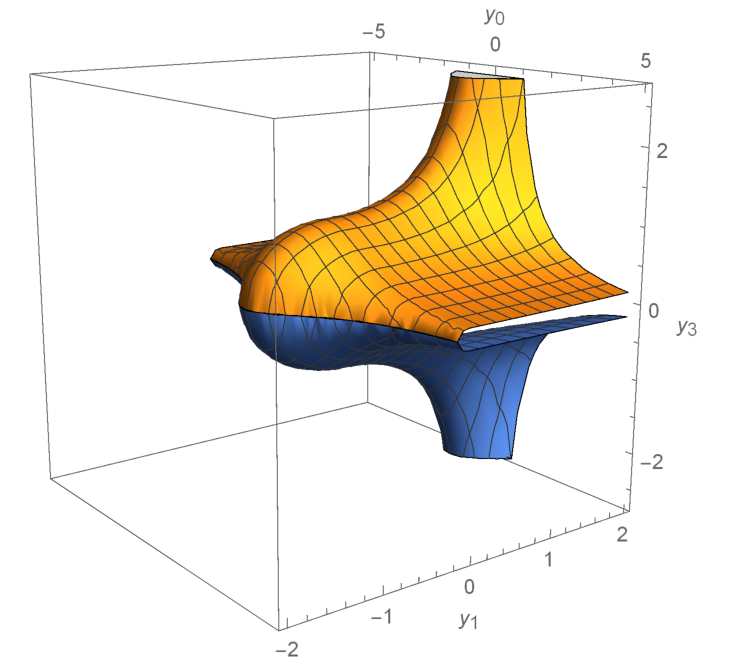
\includegraphics[width=0.562\linewidth]{Hole_with_matter_embedding.pdf}
	\caption{\label{pic_emb}The section $y^4 = y^5 = 0$ in the coordinates $ y^0 $, $ y^1 $ and $ y^3 $.}
\end{figure}

\bibliographystyle{my3beznazv}
\bibliography{paston-grav-e}
\end{document}